% Copyright Luke Olson 2009--2014
% This work is licensed under the Creative Commons
% Attribution-NonCommercial-NoDerivatives 4.0 International License. To view a
% copy of this license, visit http://creativecommons.org/licenses/by-nc-nd/4.0/.
%
\documentclass[10pt]{beamer}
%\documentclass[handout,10pt]{beamer}
%pdflatex -jobname lecture15.print lecture15
%
\mode<presentation>
{
  \usetheme[secheader]{Boadilla}
  \usefonttheme[onlymath]{serif}
  \setbeamercovered{invisible}
  \usecolortheme{luke}
  %\setbeamercovered{transparent}
  %
}
\mode<handout>
{
  \usetheme[secheader]{Boadilla}
  \usefonttheme[onlymath]{serif}
  \setbeamercovered{invisible}
  \usecolortheme{luke2}
  %\setbeamercovered{transparent}
}
\usepackage{pgf,pgfarrows,pgfnodes,pgfautomata,pgfheaps,pgfshade}
\usepackage{pxfonts}
\usepackage{eulervm}
\usepackage{listings}
%\usepackage{pgfpages}
%\pgfpagesuselayout{2 on 1}[letterpaper]
%
%
%%%%%%%%%%%%%%%%%%%%%%%%%%%%%%%%%%%%%%%%%%%%%%%%%%%%%%%%%%%%%%%%%%%%%%%%


%
%
%
\newcommand{\vb}{{\bf{b}}}
\newcommand{\ve}{{\bf{e}}}
\newcommand{\vg}{{\bf{g}}}
\newcommand{\vp}{{\bf{p}}}
\newcommand{\vr}{{\bf{r}}}
\newcommand{\vu}{{\bf{u}}}
\newcommand{\vx}{{\bf{x}}}
\newcommand{\vz}{{\bf{z}}}
\newcommand{\vA}{{\bf{A}}}
\newcommand{\vU}{{\bf{U}}}
\newcommand{\mO}{{\mathcal{O}}}
\newcommand{\mF}{{\mathcal{F}}}
\definecolor{mygray}{rgb}{0.95,0.95,0.95}
\lstset{
        language=matlab,
        numbers=left, numberstyle=\tiny, stepnumber=1, numbersep=5pt,
        basicstyle=\color{black}\ttfamily\small,
        commentstyle=\color{green}\ttfamily,
        keywordstyle=\color{blue}\ttfamily,
        stringstyle=\color{red}\ttfamily,
        showstringspaces=false,
        backgroundcolor=\color{mygray},
        breaklines,
}
\newcommand{\norm}[1]{{\ensuremath{{\|#1\|}}}}
\newcommand{\matdim}[2]{\ensuremath{#1\times#2}}
\newcommand{\rank}[1]{\ensuremath{\mathrm{rank}(#1)}}
\newcommand{\epsm}{\ensuremath{\varepsilon_m}}
\newcommand{\cmd}[1]{{\normalfont\ttfamily\bfseries#1}}

%\author{L. Olson}
\author{L. Olson}
\institute[UIUC]
{Department of Computer Science\\
University of Illinois at Urbana-Champaign\\
\vspace{0.5cm}
}
%%%%%%%%%%%%%%%%%%%%%%%%%%%%%%%%%%%%%%%%%%%%%%%%%%%%%%%%%%%%%%%%%%%%%%%%
\pgfdeclareimage[height=0.5cm]{university-logo}{./figs/uiuclogo}
\logo{\pgfuseimage{university-logo}}
%%%%%%%%%%%%%%%%%%%%%%%%%%%%%%%%%%%%%%%%%%%%%%%%%%%%%%%%%%%%%%%%%%%%%%%%
\title[CS 357]{Lecture 17}
\subtitle{Integration: Newton Cotes}
\date{October 22, 2009}

\begin{document}
% -------------------------------------------------
\begin{frame}
  \titlepage
\end{frame}
% -------------------------------------------------
%%%%%%%%%%%%%%%%%%%%%%%%%%%%%%%%%%%%%%%%%%%
\begin{frame}
\frametitle{Next...}
\begin{itemize}
  \item We can interpolate $f(x)$
  \item Can we integrate $f(x)$?
\end{itemize}
\end{frame}
%%%%%%%%%%%%%%%%%%%%%%%%%%%%%%%%%%%%%%%%%%%
%%%%%%%%%%%%%%%%%%%%%%%%%%%%%%%%%%%%%%%%%%%
\begin{frame}
\frametitle{Why?}
\begin{itemize}
  \item Often $f(x)$ is only known implicitly (known at a certain number of
points)
\vspace{1cm}

  \item Often the anti-derivative of $f(x)$ is not known.
\end{itemize}
\end{frame}
%%%%%%%%%%%%%%%%%%%%%%%%%%%%%%%%%%%%%%%%%%%
%%%%%%%%%%%%%%%%%%%%%%%%%%%%%%%%%%%%%%%%%%%
\begin{frame}
\frametitle{Integrals}
We seek a solution to the following quantity
\begin{equation*}
  \int_{a}^{b} f(x) \,dx
\end{equation*}
The Fundamental Theorem of Calculus states that 
\begin{equation*}
  \int_{a}^{b} f(x) \,dx = F(b) - F(a)
\end{equation*}
where $F$ is the antiderivative of $f$.  We don't know $F$, so we
approximate the integral operation.
\end{frame}
%%%%%%%%%%%%%%%%%%%%%%%%%%%%%%%%%%%%%%%%%%%
%% WDG - Consider using P_n insted of P for the partition into n intervals.
%%%%%%%%%%%%%%%%%%%%%%%%%%%%%%%%%%%%%%%%%%%
\begin{frame}
\frametitle{Integration}
What is the integral $\int_{a}^{b}$?
\begin{itemize}
  \item Let $P$ be a partition of $[a,b]$ of $n+1$ distinct and ordered
points with $x_0 = a$ and $x_n =b$.
  \item For interval $[x_i,x_{i+1}]$ let $m_i$ be a lower bound on $f(x)$
  \item For interval $[x_i,x_{i+1}]$ let $M_i$ be an upper bound on $f(x)$
  \item Lower Sum:
  \begin{equation*}
  L(f;P) = \sum_{i=0}^{n-1} m_i (x_{i+1}-x_i)
\end{equation*}
  \item Upper Sum:
  \begin{equation*}
  U(f;P) = \sum_{i=0}^{n-1} M_i (x_{i+1}-x_i)
\end{equation*}
\end{itemize}
\end{frame}
%%%%%%%%%%%%%%%%%%%%%%%%%%%%%%%%%%%%%%%%%%%
%%%%%%%%%%%%%%%%%%%%%%%%%%%%%%%%%%%%%%%%%%%
\begin{frame}
\frametitle{Integration}
\begin{itemize}
  \item The low sum always under-approximates the integral
  \item The upper sum always over-approximates the integral
  \begin{equation*}
  L(f;P) \leq \int_{a}^{b} f(x)\,dx \leq U(f;P)
\end{equation*}
  \item In the limit, they are equal
  \begin{equation*}
  \lim_{n\rightarrow\infty} L(f;P) = \int_{a}^{b} f(x)\,dx = \lim_{n\rightarrow\infty} U(f;P)
\end{equation*}
\end{itemize}
\end{frame}
%%%%%%%%%%%%%%%%%%%%%%%%%%%%%%%%%%%%%%%%%%%
%%%%%%%%%%%%%%%%%%%%%%%%%%%%%%%%%%%%%%%%%%%
\begin{frame}
\frametitle{Graphically: Integral}
\begin{center}
  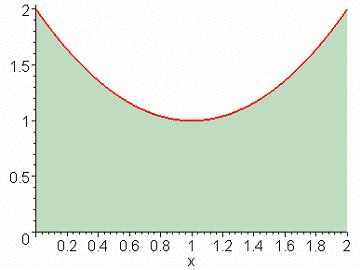
\includegraphics[height=6cm]{./figs/integral}
\end{center}
\end{frame}
%%%%%%%%%%%%%%%%%%%%%%%%%%%%%%%%%%%%%%%%%%%
%%%%%%%%%%%%%%%%%%%%%%%%%%%%%%%%%%%%%%%%%%%
\begin{frame}
\frametitle{Graphically: Lower sum}
\begin{center}
  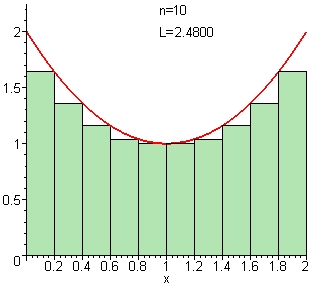
\includegraphics[height=6cm]{./figs/lowersum}
\end{center}
\end{frame}
%%%%%%%%%%%%%%%%%%%%%%%%%%%%%%%%%%%%%%%%%%%
%%%%%%%%%%%%%%%%%%%%%%%%%%%%%%%%%%%%%%%%%%%
\begin{frame}
\frametitle{Graphically: Upper sum}
\begin{center}
  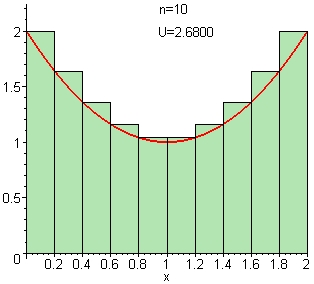
\includegraphics[height=6cm]{./figs/uppersum}
\end{center}
\end{frame}
%%%%%%%%%%%%%%%%%%%%%%%%%%%%%%%%%%%%%%%%%%%
%%%%%%%%%%%%%%%%%%%%%%%%%%%%%%%%%%%%%%%%%%%
\begin{frame}
\frametitle{Left-Riemann, Right-Riemann, Mid-Point}
\begin{itemize}
  \item The upper and lower bounds are often difficult to identify
  \item Use Left-Riemann, Right-Riemann, and Middle Riemann Sums
  \item Generally the Riemann sum is
\begin{equation*}
  S = \sum_{i=0}^{n-1} f(z_i)(x_{i+1}-x_{i})
\end{equation*}
  for $x_i \le z_i \le x_{i+1}$
  \item $z_i = x_i$ is a Left Riemann Sum
  \item $z_i = x_{i+1}$ is a Right Riemann Sum
  \item $z_i = \frac{x_{i+1}+x_{i}}{2}$ is a Middle Riemann Sum
\end{itemize}
\end{frame}
%%%%%%%%%%%%%%%%%%%%%%%%%%%%%%%%%%%%%%%%%%%
%%%%%%%%%%%%%%%%%%%%%%%%%%%%%%%%%%%%%%%%%%%
\begin{frame}
\frametitle{Goals}
We have a way to compute integrals.  Why aren't we done?

We may need to compute zillions of integrals or we may need to
accurately compute integrals in very short times to meet a real-time
requirement. 

\begin{itemize}
  \item Trapezoid Rule
  \item Composite Trapezoid Rule
  \item Simpson Rule
  \item Composite Simpson Rule
  \item Newton-Cotes in general
  \item Section 5.2 in NMC
\end{itemize}
\end{frame}
%%%%%%%%%%%%%%%%%%%%%%%%%%%%%%%%%%%%%%%%%%%
%%%%%%%%%%%%%%%%%%%%%%%%%%%%%%%%%%%%%%%%%%%
\begin{frame}
\frametitle{Trapezoid}
Goal:  Approximate
\begin{equation*}
\int_a^b f(x)\,dx
\end{equation*}
Goal:  Approximate area under $f(x)$.
\begin{itemize}
\item Old Idea: Left,Right,Midpoint Riemann integration approximate $f(x)$
by a constant function and obtain the area under the constant function.
\item New Idea: Trapezoid approximates $f(x)$ by a linear function
(degree one polynomial) and obtains the area under the linear function.
\end{itemize}
\end{frame}
%%%%%%%%%%%%%%%%%%%%%%%%%%%%%%%%%%%%%%%%%%%
%%%%%%%%%%%%%%%%%%%%%%%%%%%%%%%%%%%%%%%%%%%
\begin{frame}
\frametitle{Basic Trapezoid}
Use endpoints $[a,b]$ to obtain a linear approximation to $f(x)$.  The
area under this function is the area of a trapezoid:
\begin{equation*}
  \int_a^b f(x) \,dx \approx \frac{1}{2}(b-a)(f(a)+f(b))
\end{equation*}
\begin{center}
  \pgfimage[height=3.5cm]{./figs/basictrapezoid1}
\qquad
  \pgfimage[height=3.5cm]{./figs/basictrapezoid2}
\end{center}
\end{frame}
%%%%%%%%%%%%%%%%%%%%%%%%%%%%%%%%%%%%%%%%%%%
%%%%%%%%%%%%%%%%%%%%%%%%%%%%%%%%%%%%%%%%%%%
\begin{frame}
\frametitle{Basic Trapezoid}
\begin{itemize}
\item Trapezoid Rule:  \[\int_{x_1}^{x_2} f(x) \, dx \approx \int_{x_1}^{x_2} P_1(x)\,dx = \frac{1}{2}(f_1+f_2)h\]
\end{itemize}
 \[\int_{x_1}^{x_2} f(x) \, dx  \approx \frac{1}{2}(f_1+f_2)h \mbox{ , where } f(x) = 15\,x^2\]
\begin{example}
\[\int_{1}^{2} 15\,x^2 \approx \frac{1}{2}(15*1^2 + 15*2^2)*1\]
\[= \frac{1}{2}(15+60) = 37.5\]
\end{example}
\begin{itemize}
\item Analytical answer is $\int_{1}^{2} 15\,x^2 = \left. 5\,x^3 \right|_1^2  = 40 - 5 = 35$.
\end{itemize}
\end{frame}
%%%%%%%%%%%%%%%%%%%%%%%%%%%%%%%%%%%%%%%%%%%
%%%%%%%%%%%%%%%%%%%%%%%%%%%%%%%%%%%%%%%%%%%
\begin{frame}
\frametitle{Composite Trapezoid}
Obviously a naive linear approximation won't cut it.
\bigskip

Consider a partition $P=\{x_0=a< \dots x_n = b\}$ of $[a,b]$.
\bigskip

In each interval $[x_i,x_{i+1}]$ use the basic Trapezoid:
\begin{equation*}
  \int_a^b f(x)\,dx \approx \sum_{i=0}^{n-1}
\frac{1}{2}(x_{i+1}-x_{i})(f(x_i)+f(x_{i+1}))
\end{equation*}

\begin{center}
  \pgfimage[height=3.5cm]{./figs/comptrapezoid1}
\qquad
  \pgfimage[height=3.5cm]{./figs/comptrapezoid2}
\end{center}

\end{frame}
%%%%%%%%%%%%%%%%%%%%%%%%%%%%%%%%%%%%%%%%%%%
%%%%%%%%%%%%%%%%%%%%%%%%%%%%%%%%%%%%%%%%%%%
\begin{frame}[fragile]
\frametitle{Composite Trapezoid}
\begin{itemize}
  \item With uniform spacing of $P$, $h_i=x_{i+1}-x_{i}=h$ is constant
\begin{equation*}
T(f;P) = \int_a^b f(x)\,dx \approx \frac{h}{2}\sum_{i=0}^{n-1}f(x_i)+f(x_{i+1})
\end{equation*}
  \item This becomes
\begin{equation*}
T(f;P) = \int_a^b f(x)\,dx \approx \frac{h}{2}\left(f(x_0) + 2 f(x_1) +
2f(x_2) + \dots + 2 f(x_{n-1}) + f(x_n)\right)
\end{equation*}
\end{itemize}
\begin{lstlisting}[mathescape]
$h = (b-a)/n$
$sum = (f(a)+f(b))/2$
for $i=1$ to $n-1$
  $sum = sum + f(x_i)$
end
$sum = sum \cdot h$
\end{lstlisting}
\end{frame}
%%%%%%%%%%%%%%%%%%%%%%%%%%%%%%%%%%%%%%%%%%%
%%%%%%%%%%%%%%%%%%%%%%%%%%%%%%%%%%%%%%%%%%%
\begin{frame}
\frametitle{Example}
Test composite trapezoid for
\begin{equation*}
  \int_0^5 x e^{-x}
\end{equation*}

Question: What is the order of accuracy?
\bigskip

Look at $h^p$ with
\begin{equation*}
  p \approx \frac{log(err^{(k)}/err^{(k-1)})}{log(h^{(k)}/h^{(k-1)})}
\end{equation*}
\end{frame}
%%%%%%%%%%%%%%%%%%%%%%%%%%%%%%%%%%%%%%%%%%%
%%%%%%%%%%%%%%%%%%%%%%%%%%%%%%%%%%%%%%%%%%%
\begin{frame}
\frametitle{Accuracy}
So composite Trapezoid appears to be order 2.  Why?  Look first a basic Trapezoid:
\begin{equation*}
  \int_a^b f(x) \,dx \approx \frac{1}{2}(b-a)(f(a)+f(b))
\end{equation*}
Looking at the error 
\begin{align*}
  E &= \int_a^b f(x) \,dx - \int_a^b \frac{(b-x)f(a)}{b-a}+\frac{(x-a)f(b)}{b-a}\,dx\\
    &=\int_a^b \frac{(b-a)f(x) - (b-x)f(a) - (x-a)f(b)}{b-a}\,dx\\
    &=\int_a^b (x-a)(x-b)f[a,b,x]\,dx\\
    &=f[a,b,\xi]\int_a^b (x-a)(x-b)\,dx ( \text{MVT})\\
    &=\frac{f''(\eta)}{2}\left(-\frac{1}{6}(b-a)^3\right)\\
    &=-\frac{(b-a)^3 f''(\eta)}{12}
\end{align*}
\end{frame}
%%%%%%%%%%%%%%%%%%%%%%%%%%%%%%%%%%%%%%%%%%%
%%%%%%%%%%%%%%%%%%%%%%%%%%%%%%%%%%%%%%%%%%%
\begin{frame}
\frametitle{Accuracy}
What about Composite Trapezoid?
\begin{equation*}
T(f;P) = \int_a^b f(x)\,dx \approx \frac{h}{2}\sum_{i=0}^{n-1}f(x_i)+f(x_{i+1})
\end{equation*}
The error in each interval $[x_i,x_{i+1}]$ is
\begin{equation*}
E_i =-\frac{h^3 f''(\eta_i)}{12}
\end{equation*}
So the total error is
\begin{align*}
\sum_{i=0}^{n-1} E_i & = \sum_{i=0}^{n-1}  -\frac{h^3 f''(\eta_i)}{12}\\
& = -n\frac{h^3 f''(\eta)}{12} (IVT)\\
& = -\frac{(b-a) h^2 f''(\eta)}{12}
\end{align*}
\end{frame}
%%%%%%%%%%%%%%%%%%%%%%%%%%%%%%%%%%%%%%%%%%%
%%%%%%%%%%%%%%%%%%%%%%%%%%%%%%%%%%%%%%%%%%%
\begin{frame}[shrink]
\frametitle{Example}
How many points should be used to ensure the composite Trapezoid rule is
accurate to $10^{-6}$ for $\int_0^1 e^{-x^2}\,dx$?
\bigskip
Need 
\begin{equation*}
\frac{(b-a) h^2 f''(\eta)}{12} \leq 10^{-6}
\end{equation*}
How big is $f''(x)$?
\begin{align*}
  f(x) &= e^{-x^2}\\
  f'(x) &=-2xe^{-x^2}\\
  f''(x) &=-2e^{-x^2}+4x^2e^{-x^2}\\
  f'''(x) &=12xe^{-x^2}-8x^3e{-x^2}
\end{align*}
So $f'''$ is always positive.  So $f''$ is monotone increasing and thus
take on a maximum at an endpoint: $f''(0) = 2$. Then bound
\begin{equation*}
\frac{(b-a) 2 h^2}{12} \leq 10^{-6}
\end{equation*}
Or
\begin{equation*}
h^2 \leq 6 \times 10^{-6} \quad \Rightarrow \quad \sqrt{(1/6)} 10^{3} \leq n
\end{equation*}
or $n>410$.
\end{frame}
%%%%%%%%%%%%%%%%%%%%%%%%%%%%%%%%%%%%%%%%%%%
%%%%%%%%%%%%%%%%%%%%%%%%%%%%%%%%%%%%%%%%%%%
\begin{frame}
\frametitle{How do we improve Trapezoid?}
  \begin{itemize}
  \item instead of a linear approximation, use a quadratic approximation
  \item $\Rightarrow$ Simpson's Rule
\end{itemize}
\end{frame}
%%%%%%%%%%%%%%%%%%%%%%%%%%%%%%%%%%%%%%%%%%%
%%%%%%%%%%%%%%%%%%%%%%%%%%%%%%%%%%%%%%%%%%%
\begin{frame}
\frametitle{Simpson}
  \begin{itemize}
  \item consider $\int_{a}^{b} f(x)\,dx$
  \item partition $P =\{a,a+h,b=a+2h\}$
  \item or $\int_{0}^{2h} f(x)\,dx$
  \item partition $P =\{0,h,2h\}$
  \item replace $f(x)$ by a quadratic $p(x)$:
    \begin{align*}
      f(x) & \approx p(x)\\
           & = f(0) + \frac{f(h)-f(0)}{2} x + \frac{f(2h)-2f(h)-f(0)}{2h^2} x (x-h)\\
          & = \text{newton form}
    \end{align*}
  \item integrate $\int_{0}^{2h} p(x)\,dx$:
  \begin{align*}
  \int_{0}^{2h} f(x)\,dx &\approx \int_{0}^{2h} p(x)\,dx\\
                         &= \frac{h}{3}\left[f(0) + 4f(h) + f(2h)\right]
  \end{align*}
        
\end{itemize}
\end{frame}
%%%%%%%%%%%%%%%%%%%%%%%%%%%%%%%%%%%%%%%%%%%
%%%%%%%%%%%%%%%%%%%%%%%%%%%%%%%%%%%%%%%%%%%
\begin{frame}
\frametitle{Simpson}
Since $b-a=2h$ we have
\begin{block}{basic Simpson's Rule}
  \begin{equation*}
  \int_{a}^{b} f(x)\,dx \approx \frac{b-a}{6}\left[f(a) + 4f\left(\frac{a+b}{2}\right) + f(b)\right]
  \end{equation*}
\end{block}
\begin{center}
  \pgfimage[height=4.5cm]{./figs/basicsimpson1}
\end{center}
\end{frame}
%%%%%%%%%%%%%%%%%%%%%%%%%%%%%%%%%%%%%%%%%%%
%%%%%%%%%%%%%%%%%%%%%%%%%%%%%%%%%%%%%%%%%%%
\begin{frame}
\frametitle{Composite Simpson}
Over a uniform partition $P={x_0,x_1,\dots,x_n}$, use Basic Simpson's Rule over
each subinterval $[x_{2i},x_{2i+2}]$
  \begin{align*}
  \int_{a}^{b} f(x)\,dx & = \sum_{i=0}^{n/2-1} \int_{x_{2i}}^{x_{2i+2}} f(x)\,dx\\
                        & = \sum_{i=0}^{n/2-1} \frac{2h}{6}\left[f(x_{2i}) + 4f(x_{2i+1}) + f(x_{2i+2})\right]\\
                        & = \frac{h}{3}\left[f(x_{0}) + 4f(x_1) + 2f(x_2) + 4f(x_3) + 2f(x_4) + \dots + 4f(x_{n-1}) +f(x_{n})\right]
  \end{align*}
\end{frame}
%%%%%%%%%%%%%%%%%%%%%%%%%%%%%%%%%%%%%%%%%%%
%%%%%%%%%%%%%%%%%%%%%%%%%%%%%%%%%%%%%%%%%%%
\begin{frame}
\frametitle{Simpson}
\begin{block}{Composite Simpson's Rule}
  \begin{equation*}
  \int_{a}^{b} f(x)\,dx \approx \frac{h}{3}\left[f(a) + f(b) + 4 \sum_{i=1}^{n/2} f(a+(2i-1)h) + 2\sum_{i=1}^{n/2 - 1}f(a+2ih)\right]
  \end{equation*}
\end{block}
\begin{center}
  \pgfimage[height=4.5cm]{./figs/compsimpson1}
\end{center}
\end{frame}
%%%%%%%%%%%%%%%%%%%%%%%%%%%%%%%%%%%%%%%%%%%
%%%%%%%%%%%%%%%%%%%%%%%%%%%%%%%%%%%%%%%%%%%
\begin{frame}
\frametitle{Simpson}
How accurate is Simpson?
\bigskip
Recall composite Trapezoid: $I - T(f,P) = -\frac{1}{12}(b-a)h^2f''(\xi) - \mO(h^2)$
\bigskip

Prediction? $\mO(h^2)$?\quad $\mO(h^3)$?\quad $\mO(h^4)$?
\bigskip

\texttt{int\_simpson\_test.m}
\end{frame}
%%%%%%%%%%%%%%%%%%%%%%%%%%%%%%%%%%%%%%%%%%%
%%%%%%%%%%%%%%%%%%%%%%%%%%%%%%%%%%%%%%%%%%%
\begin{frame}
\frametitle{Why is composite Simpson $\mO(h^4)$?}
Taylor Series:
\begin{align*}
f(a+h) & = f + hf' + \frac{1}{2!}h^2 f'' + \frac{1}{3!}h^3 f''' + \frac{1}{4!}h^4 f^{(4)} + \frac{1}{5!}h^5 f^{(5)} + \dots\\
f(a+2h) & = f + 2hf' + 2h^2 f'' + \frac{4}{3}h^3 f''' + \frac{2}{3}h^4 f^{(4)} + \frac{4}{15}h^5 f^{(5)} + \dots\\
\end{align*}
This gives
\begin{equation*}
\frac{h}{3}\left[f(a)+4f(a+h)+f(b)\right] = 2hf +2h^2f' + \frac{4}{3}h^3f''+\frac{2}{3}h^4f'''+\frac{5}{18}h^5f^{(4)}
\end{equation*}
Integrating the Taylor Series expansion of $f(x)$ exactly gives
\begin{equation*}
\int_{a}^{b}f(x)\,dx = 2hf +2h^2f' + \frac{4}{3}h^3f''+\frac{2}{3}h^4f'''+\frac{4}{15}h^5f^{(4)}
\end{equation*}
So basic Simpson's Rule gives an error of
\begin{equation*}
-\frac{1}{90}\left(\frac{b-a}{2}\right)^5 f^{(4)}(\xi)
\end{equation*}
\end{frame}
%%%%%%%%%%%%%%%%%%%%%%%%%%%%%%%%%%%%%%%%%%%
%%%%%%%%%%%%%%%%%%%%%%%%%%%%%%%%%%%%%%%%%%%
\begin{frame}
\frametitle{Why is composite Simpson $\mO(h^4)$?}
basic Simpson's Rule:
\begin{equation*}
-\frac{1}{90}\left(\frac{b-a}{2}\right)^5 f^{(4)}(\xi)
\end{equation*}
Over $n/2$ subintervals $[x_{2i},x_{2i+2}]$ becomes:
\begin{align*}
err & =  \sum_{i=1}^{n/2} -\frac{1}{90}\left(\frac{x_{2i+2}-x_{2i}}{2}\right)^5 f^{(4)}(\xi_i)
      = -\frac{1}{90}  \sum_{i=1}^{n/2} \left(\frac{2h}{2}\right)^5 f^{(4)}(\xi_i)\\
    & = -\frac{1}{90}  \frac{n}{2}h^5 f^{(4)}(\xi)
      = -\frac{1}{180} \frac{(b-a)}{h}h^5 f^{(4)}(\xi)\\
    & = -\frac{b-a}{180} h^4 f^{(4)}(\xi)
\end{align*}
\vspace{-0.5cm}

\begin{block}{Composite Simpson's Rule}
\begin{equation*}
  -\frac{b-a}{180}h^4 f^{(4)}(\xi)
\end{equation*}
\end{block}
We ``gain'' two orders over Trapezoid
\end{frame}
%%%%%%%%%%%%%%%%%%%%%%%%%%%%%%%%%%%%%%%%%%%
%%%%%%%%%%%%%%%%%%%%%%%%%%%%%%%%%%%%%%%%%%%
\begin{frame}
\frametitle{Can we generalize?}
Summary:
\begin{itemize}
  \item left/right Riemann: approximate $f(x)$ by 0-degree $p(x)$ and integrate
  \item Trapezoid: approximate $f(x)$ by 1-degree $p(x)$ and integrate
  \item Simpson: approximate $f(x)$ by 2-degree $p(x)$ and integrate
\end{itemize}
\begin{block}{Degree of Precision} % according to Atkinson
  If the integration rule has zero error when integrating any polynomial of
degree $\leq r$
\smallskip

and
\smallskip

If the error is nonzero for some polynomial of degree $r+1$,

and
\smallskip

then, the rule has \emph{degree of precision} equal to $r$.
\end{block}
\end{frame}
%%%%%%%%%%%%%%%%%%%%%%%%%%%%%%%%%%%%%%%%%%%
%%%%%%%%%%%%%%%%%%%%%%%%%%%%%%%%%%%%%%%%%%%
\begin{frame}
(basic) Newton-Cotes rules:
\begin{tabular}{l l l}
name & $n$ & formula \\\hline
Trapezoid       & 1 & $\frac{(b-a)}{2}\left[f(a) + f(b)\right]$\\[5pt]
Simpson's $1/3$ & 2 & $\frac{(b-a)}{6}\left[f(a) + 4f(\frac{a+b}{2}) + f(b)\right]$\\[5pt]
Simpson's $3/8$ & 3 & $\frac{(b-a)}{8}\left[f(a) + 3f(a+h) + 3f(b-h) + f(b)\right]$\\[5pt]
Boole's         & 4 & $\frac{(b-a)}{90}\left[7f(a) + 32f(a+h) + 12f(\frac{a+b}{2}) + 32f(b-h)+7f(b)\right]$\\[5pt]
\end{tabular}
\bigskip

Error bounds for composite Newton-Cotes:
\begin{tabular}{l l l l}
name & $n$ & error & $h$\\\hline
Trapezoid       & 1 & $-\frac{(b-a)h^2}{12}f''(\xi)$ & $h=b-a$\\[5pt]
Simpson's $1/3$ & 2 & $-\frac{(b-a)h^4}{90}f^{(4)}(\xi)$ & $h=(b-a)/2$\\[5pt]
Simpson's $3/8$ & 3 & $-\frac{(b-a)h^4}{80}f^{(4)}(\xi)$ & $h=(b-a)/3$\\[5pt]
Boole's         & 4 & $-\frac{2(b-a)h^6}{945}f^{(6)}(\xi)$ & $h=(b-a)/4$\\[5pt]
\end{tabular}

\end{frame}
%%%%%%%%%%%%%%%%%%%%%%%%%%%%%%%%%%%%%%%%%%%
\end{document}
